\chapter{书面翻译}

\section{基于编码树剪枝的HEVC快速编码单元推断方法}

\title{基于编码树剪枝的HEVC快速编码单元推断方法}

{\heiti 摘要:} 本文为HEVC提出了一种快速决定编码单元划分的方法,这是一种通过基于树剪枝的
策略,来更早推断出编码单元的尺寸的方法。在HEVC中,最为有效的是可变的编码单元尺寸,这是一个
全新的概念。在推断最佳的编码单元尺寸的过程中,作为参考的HEVC编码器会逐个测试每种可能的编码
单元尺寸,以便估测每种情况下,由编码单元尺寸所决定的编码器的表现。在整个编码过程中,这是
主要的计算复杂度来源,因此,为了实现一个高效快速的编码器,这一过程应是攻坚的重点。一种简单的
树剪枝算法是,若当前节点的编码模式已经足够好,那么其子节点的计算均可以被跳过(例如SKIP模式)。
实验结果显示,本文所提出的方法,相较于测试模型3.0下的HEVC编码器,最多有可能达到40 \% 的
时间缩减,而其代价仅仅是一点可以忽略不计的编码效果上的损失。在第六次JCT-VC会议上,本文所提出
的方法被HEVC编码器测试模型4.0所采用。

{\heiti 关键词:} HEVC;编码单元早推断;快速高效视频编码;视频编码。

\subsection{引言}

2010年,ISO/IEC旗下的组织MEPG和ITU-T旗下的VCEG拟定了一份新的视频编码标准,该标准被称为HEVC。
这份新标准被期望能够满足人们对于视频日益增长的需求,包括压缩效率、视频分辨率、帧率、计算复杂度
等诸多方面。尽管HEVC标准尚处于发展阶段,迄今为止,其压缩效率已经达到了前一标准(MPEG-4 AVC/H.264)
的二倍之高。

虽然HEVC遵循传统的编码结构,包括基于块的运动补偿和变换编码,但实质性改进来自于基于四叉树结构的
新的分层编码概念。在HEVC中,视频编码和解码过程由以下三个单元组成:编码单元(CU),用于作为变换四叉树
的根,以及用于帧间/跳过/帧内预测;预测单元(PU),用于决定模式,包括运动估计和率失真优化;变换
单元(TU),用于变换编码和熵编码。在三种编码单元中,CU对于提升压缩效率是至关重要、最为关键的,
因为它决定了初始编码块的大小,而初始编码块的大小对其他处理单元(例如,PU和TU)的性能影响很大。

当使用CU、PU和TU三种编码单元时,提升压缩效率是可能的,但同时,这也会显着地增加计算的复杂度。通常,
在编码过程中会生成一个四叉树,其中根节点表示最大的CU大小,并且具有对应于下一个CU大小的四个子节点。
这棵树被称为编码树,且其最大深度为4。编码单元与编码树(例如,当根节点的CU大小为64 x 64且树的深度
设定为4的时候,CU0大小为64 x 64,CU1为32 x 32,...,CU3为8 x 8。)被包含在CU尺寸优化的计算与选择中,
这一点导致了CU数量的指数增长(例如,1 x CU0 + 4 x CU1 + 16 x CU2 + 64 x CU3),这一点被直观
地展示在 \ref {fig:trans-cu-demo} 中。由于每一个CU都对应着一个相应的PU和TU的计算,因此,日益
增长的计算复杂对给实时编码器的设计带来了了严峻的挑战。HEVC参考编码器(即,3.0版)大约比MPEG-4 
AVC/H.264参考编码器(即,JM 17.0 高配置版本)慢三倍。为了克服HEVC编码器在计算上的复杂性,我们
提出了基于CU早终止的树剪枝策略,并在JCT-VC第六会议上介绍了该方法。

\begin{figure}[H] % use float package if you want it here
  \centering
  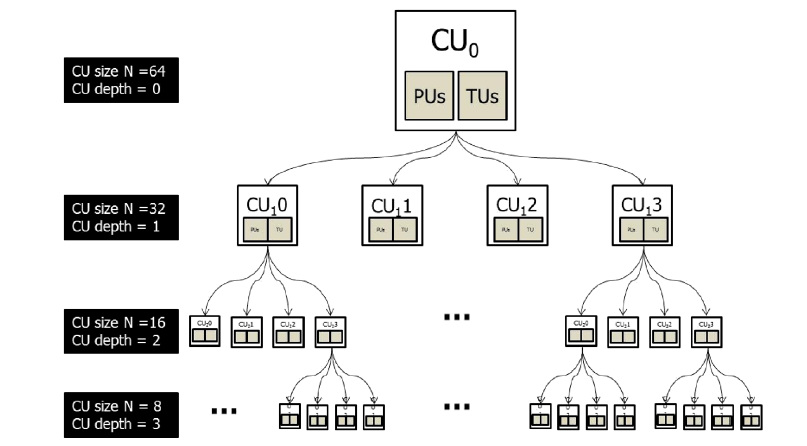
\includegraphics[width = \textwidth]{trans-cu-demo}
  \caption{根节点CU为64 x 64、深度为4的编码树结构示意图}
  \label{fig:trans-cu-demo}
\end{figure}


\subsection{基于树剪枝的快速编码单元推断}

基于可变CU大小的编码树推断过程计算复杂度可以描述如下:

\begin{equation}
\label{eq-cu-complexity}
\left\{\begin{array}{l}
f(n) = f(n - 1) + 4^n * M_n, f(0) = M_0 \;\; and \\
M_i = {(\frac14)}^i * M_{i - 1}
\end{array}\right.
\end{equation}

这里,$f(n)$ 是当编码树的最大深度被设定为 $n$ 时所需操作的总数,而 $M_i$ 则是
对于第 $i$ 层给定的CU大小所需的操作总数。在 \ref{eq-cu-complexity} 中,我们假定 $M_i$ 是
$M_{i-1}$ 的四分之一是因为CU的大小比起前一层会减少四分之一。总的操作数可以被整合为如下的
公式:

\begin{equation}
\label{eq-cu-complexity-comb}
f(n) = \sum_{i=0}^n 4^i * M_i \cong \mathcal{O} (M_0 * n)
\end{equation}

如 \ref{eq-cu-complexity-comb} 所展示,计算的复杂度随着CU深度的增加单调增加。当考虑到 $M_i$
代表着包括对每个CU大小的运动估计在内的整个编码过程这一事实,最大CU深度就自然成为了决定编码时间
的主要因素。

本文研究了一种通过更早地确定CU的深度来加速CU深度推断的策略。我们利用了这样一个事实,当当前CU节点
的代价低于该节点子节点的代价时,我们就不必再对子树进行进一步的处理(例如,$RDCost(CU_t) < \sum_{i=0}^3 RDCost(CU^i_{t-1})$)。
这一方法的唯一问题是,子树的代价必须是已知的,这一要求妨碍了子树计算复杂度的减少程度。我们可以避免
子树代价的计算,如果当前节点的代价已经是最小的了(例如,SKIP模式),而这正是本方法的核心概念。
为了进一步减少计算复杂度,我们可以定义剪枝的条件如下:

\begin{equation}
\label{eq-pruning-condition}
\begin{split}
Pruning & \; codition: \\
(\mathop{m'} & =  \mathop{argmin}\limits_{m \in Mode} RDCost(CU_t | PU=m)) \le Threshold \\
Mode & = \{ SKIP, Inter2Nx2N, Inter2NxN, InterNx2N, InterNxN \} 
\end{split}
\end{equation}

这里,Mode表示按根据复杂度确定的预测模式的有序集合,而 $\mathop{m'}$ 则是为当前CU深度选择的
预测模式,且Threshold将根据Mode选择。在 \ref{eq-pruning-condition} 中,通过从SKIP到InterNxN,不断
改变Threshold的值,剪枝过程的可能性将被推断。若Threshold被设置为SKIP时,剪枝过程将不会对压缩效率产生
影响;否则,以降低压缩效率为代价,更多的子树将被剪去。根据上述分析,我们提出了 \ref{trans-algorithm} 
所示的剪枝过程。


\begin{figure}[H] % use float package if you want it here
  \centering
  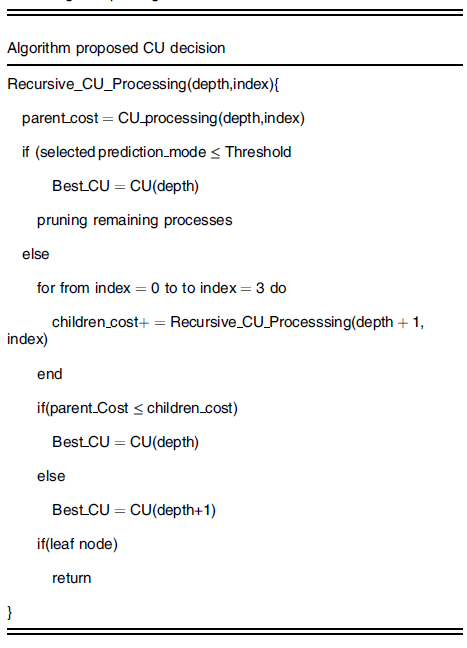
\includegraphics[width = 0.6\textwidth]{trans-algorithm}
  \caption{基于树剪枝的CU推断方法的步骤}
  \label{fig:trans-algorithm}
\end{figure}

\subsection{实验结果}

为了进行性能评测,我们测试了了我们的方法与HM 3.0两种方法的总执行时间,以确认计算复杂度的降低
程度。编码的表现以 $\Delta Bitrate[ (B_{PRO} - B_{REF})/B_{REF} X 100 ]$ 和 
$ \Delta PSNR(P_{PRO} - P_{REF})$ 来衡量,并且时间的减少以 $ \Delta Time[ (T_{PRO} - T_{REF})/T_{REF} X 100 ]$
来衡量。在实验中,我们吧Threshold值设置为SKIP模式。有关编码环境的更多细节在 \ref{fig:trans-cfg} 被展示。

\begin{figure}[H] % use float package if you want it here
  \centering
  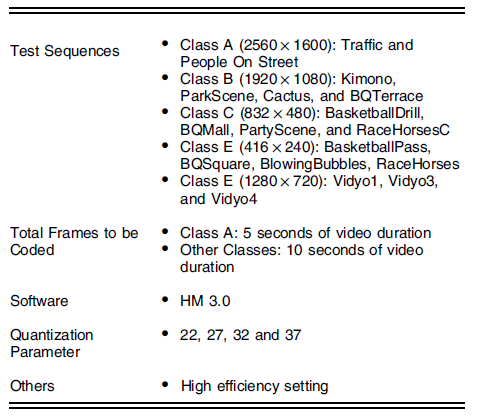
\includegraphics[width = 0.6\textwidth]{trans-cfg}
  \caption{测试环境与软件参考配置}
  \label{fig:trans-cfg}
\end{figure}

\begin{figure}[H] % use float package if you want it here
  \centering
  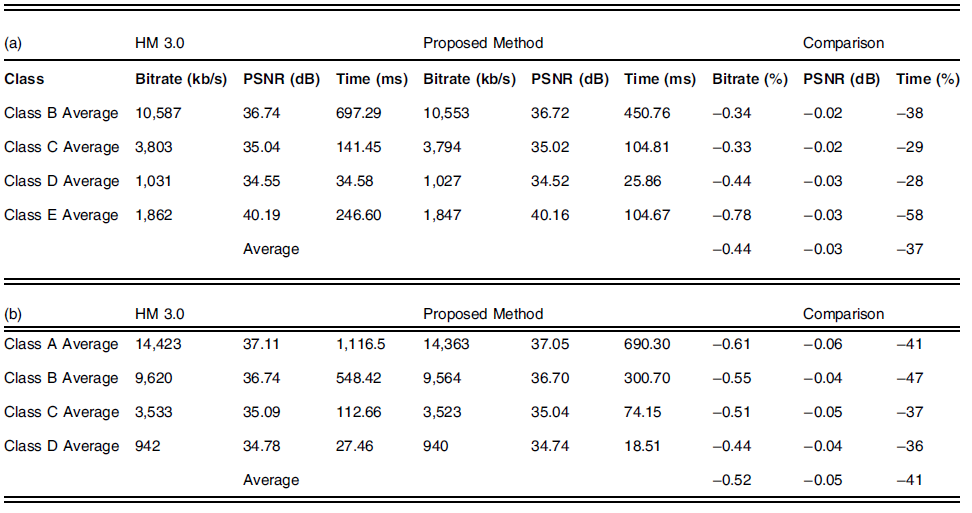
\includegraphics[width = \textwidth]{trans-result}
  \caption{文中所提出的算法与HM3.0在编码时间上的对比:(a)低延迟方案;(b)随机访问方案}
  \label{fig:trans-result}
\end{figure}

\ref{fig:trans-result} 展示了在低延迟方案与随机访问方案两种环境下,我们评测了我们的方法与
HM 3.0两种方法的总执行时间。尽管我们测试了每一种 \ref{fig:trans-cfg} 中所列举的不同的量化参数下的结果,
但 \ref{fig:trans-result} 中,我们只展示每一类的平均结果。 \ref{fig:trans-result} 显示了我们的
方法相较于HM 3.0,,在低延迟方案的环境下减少了63.34\%的时间,而在随机访问方案的环境下,则减少了
59.43 \%的时间。以图像质量的轻微退化为代价所获得的编码增益,是所提出的方法的自然结果,因为编码树修剪过程
会使图像质量上的比特减少。通过调整Threshold的值,我们可以节约更多的编码时间,但其代价是图片质量
的进一步下降。目前,我们所提出的方法,在模式设置为SKIP时,能得到编码时间与图片质量相平衡的最好结果。


\subsection{结论}

在本文中,我们为HEVC提出了一种快速的CU决策方法,这种方法基于编码树修剪从而更早确定CU的大小,与HM 3.0
编码器相比,仅以可以忽略不计的BD-比特率损失为代价,就可以使编码时间减少约40 \%。实验结果表明,当你想设计
一个快速的HEVC编码器时,我们所提出的编码树剪枝方法应当被考虑。在JCT-VC第六次会议上,HEVC测试模型4.0
编码器采用了我们所提出的方法。

\subsection*{References}

\begin{translationbib}
  \item Choi, Kiho, Sang-Hyo Park, and Euee S. Jang. "Coding tree pruning based CU early termination." 
  JCTVC-F092, Torino, Italy (2011): 14-22.
\end{translationbib}



\section{一种有效的H.264上的可变块大小早终止算法}

\title{一种有效的H.264上的可变块大小早终止算法}

{\heiti 摘要:} H.264视频编码标准比以前的标准提供了更高的编码效率,但同时,其复杂度也显著提高。
在H.264编码器中,最耗时的组成部分是可变块大小的运动估计。为了降低运动估计的复杂度,本文提出了一种
早终止算法。它通过检查仅仅一个搜索点来预测最佳的运动矢量。使用该方法,一些运动搜索可以被提前停止,
由此,大量的搜索点可以被跳过。本文所提出的方法适用于任何快速运动估计算法。实验采用的是H.264所采用的
一种快速运动估计算法。结果表明,本算法显著降低了复杂度,而代价仅仅是可以忽略不计的视频质量的降低。

{\heiti 关键词:} 早终止;H.264;运动估计;可变块大小。

\subsection{引言}

近年来,视频编码技术高速发展。理所当然地,压缩性能的提升伴随着计算代价的增长。作为ITU-T的VCEG和
ISO/IEC的MPEG所最新制定标准的H.264,相较于之前的H.261、H.263、MPEG-1/2/4等标准,在编码效率上有着
巨幅的提升。然而,其过高的计算复杂度使其无法被广泛应用到实时业务中。

通常来说,一个视频编码器最为耗时的部分是运动估计。减少其计算代价的方法有两种。第一种是加速算法本身,
对ME过程来说,数种快速算法被提出,例如六边形搜索(HBS)、增强型预测分区搜索(EPZS)和混合非对称
交叉多六边形网格搜索(UMHexagonS)等。另一种方法就是更早地终止ME的计算。通过预测那些DCT系数会被量化
为0的块,一些方法有效地减少了ME的计算量。另一方面,一些块的重要部分在ME之后具有零运动矢量(MV)。
据此,有算法提出的零运动检测算法(ZMD),通过将它们的差值的绝对值求和,并与预先定义的阈值进行比较来检测这样的块,
然后跳过其余的搜索点。

然而,上述早终止方法都是针对以前的编码方案(如H.263)而开发的。它们不能再应用于H.264。这是因为相比于仅有
两中块大小(16x16和8x8)的H.263,H.264拥有从16x16到4x4变化的七种块大小。

通过扩展ZMD的概念,我们提出了一种用于H.264视频编码的可变块大小最佳运动检测(VBBMD)算法。
该方法在三个方面与ZMD不同:

\begin{enumerate}
  \item 基于不同块大小的检测精度,分别获得VBBMD中使用的阈值,同时考虑了复杂度的降低,使得阈值的决策更加合理;
  \item 在VBBMD中,除零运动点外,预测的移动到的点也会被检查,从而更多的搜索点可以被跳过;
  \item 对于16x16的块,VBBMD使用双阈值。使用较低的阈值跳过较小的块的运动搜索。
\end{enumerate}

我们的方法可以适用于任何运动搜索算法,并且不需要额外的计算。注意,整个讨论集中于帧间帧(P帧)和
整数像素运动搜索。文章的剩余部分如下进行组织。 \ref{sec:app2-early-termination} 介绍了早期终止算法
及其改进。 \ref{sec:app2-sim-result} 中给出了仿真结果。最后,在 \ref{sec:app2-conclusion} ,
我们总结了本文,并给出了未来的方向。

\subsection{早终止算法}
\label{sec:app2-early-termination}

\subsubsection{可变块大小零运动推断}

通常来说,对大多数序列,在ME后相当数量的块会有这零运动矢量,正如 \ref{fig:trans2-zmb} 展示的一样。


\begin{figure}[H] % use float package if you want it here
  \centering
  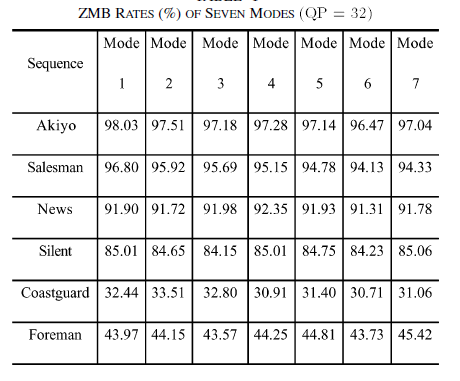
\includegraphics[width = 0.6\textwidth]{trans2-zmb}
  \caption{当量化参数为32时,七种模式下零运动块的比例}
  \label{fig:trans2-zmb}
\end{figure}

表中,模式1-7代表从16x16到4x4的七种帧间预测模式,如 \ref{fig:trans2-7-predict-mode} 所展示。

\begin{figure}[H] % use float package if you want it here
  \centering
  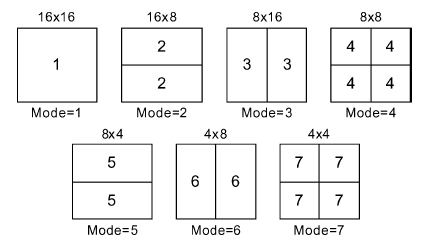
\includegraphics[width = 0.6\textwidth]{trans2-7-predict-mode}
  \caption{H.264中的七种预测模式}
  \label{fig:trans2-7-predict-mode}
\end{figure}

可以看出,不论是运动较为活跃亦或是不太活跃的视频序列,有30.71 \%到98.03\%的块存在零运动。
如果我们可以预测零运动块(ZMB),我们可以提前停止ME的计算,从而消除计算的一部分。通过扩展ZMD的概念,
我们开发了一个可变块大小的ZMD(VBZMD)算法。

在以前的ZMD方法中,当块的SAD小于给定阈值时,块可以被看作是ZMB。在H.264中选择最佳匹配块时,使用代价函数$J$
而不是SAD作为预测误差的度量。

\begin{equation}
\label{eq2-cost}
J(m, \lambda) = SAD (s, c(m)) + \lambda R(m - p)
\end{equation}

这里,$m = (m_x, m_y)^T$ 是当前的MV,$p = (p_x, p_y)^T$ 是预测的MV,而 $ \lambda $则是拉格朗日乘数,
$ R(m - p) $ 是编码MV所用的比特数。

如果一个块是零运动的,那么$MV(0, 0)$ 处极有可能有一个很小的代价值。因此,我们为七种模式分别定义阈值 
$THZ_i(i=1,...,7)$。在整个运动估计过程中,$MV(0, 0)$ 首先被检查。如果$MV(0, 0)$ 处的代价满足 \ref{eq2-thz-condition} ,
我们就认为这个块是一个ZMB,由此剩余的搜索过程既可以被停止。

\begin{equation}
\label{eq2-thz-condition}
J_i < THZ_i, \; for \; i = 1,...,7.
\end{equation}

H.264中ZMD的关键是如何去决定不同块大小下的阈值。很明显,阈值越大,检测到的ZMB越多,更多的搜索点就可以被跳过。
然而同时,更多的块被错误地选择,这会导致更大的图像质量损失。因此,在性能和复杂性之间存在一个平衡。在实践中,防止
视频质量的损失可能比复杂度的轻微增加更重要。

因此,我们将检测精度作为确定阈值的指导。这里,精度表示当代价小于阈值时,块为ZMB的概率。我们的方法是,在实验中基于
不同的准确率获得多个候选阈值集,并选择一个最优集合,在实践中,我们需要在质量和复杂度之间取一个较好的折衷。
许多序列的实验表明,在相同的阈值下,低运动场景中的准确率和检测率都高于有较多运动的场景中的准确率和检测率。
由于Foreman序列可以代表具有较大运动的场景,所以我们可以选择基于Fordman的阈值,并将它们应用到其他序列。 
\ref{fig:trans2-ac-foreman} 显示了我们获得的候选阈值。

\begin{figure}[H] % use float package if you want it here
  \centering
  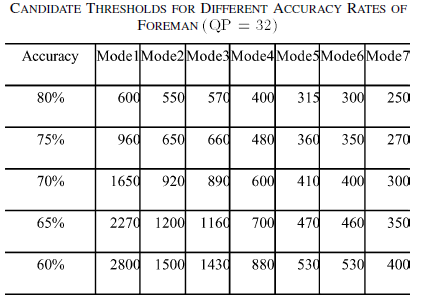
\includegraphics[width = 0.6\textwidth]{trans2-ac-foreman}
  \caption{对于Foreman序列,不同准确率的备选阈值(QP=32)}
  \label{fig:trans2-ac-foreman}
\end{figure}

在我们的方法中,如果块的零运动代价小于相应的阈值,则我们将其视为块的最佳MV并跳到同一宏块中的下一个块。如果当前块是宏块中的
最后一个块,则跳转到下一个模式。在所有模式被检查之后,拥有最小成本的模式被选择,并应用于后续的任一为H.264设计的ME算法。
在模式1中,由于一个宏块只包含一个块,如果零运动成本足够小,那么不仅可能是最好的MV,而且模式1也很可能是宏块的最佳模式。
因此,我们为模式1定义了额外的低阈值THS。如果零运动代价小于THS,则整个宏块的运动搜索停止。VBZMD的整个过程概述如下:

\begin{figure}[H] % use float package if you want it here
  \centering
  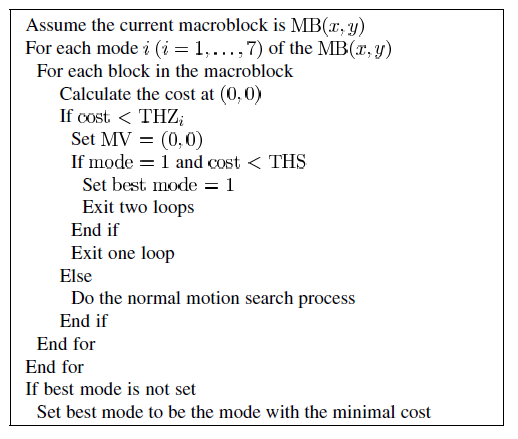
\includegraphics[width = 0.6\textwidth]{trans2-vbzmd}
  \caption{VBZMD整个过程}
  \label{fig:trans2-vbzmd}
\end{figure}

我们所使用的H.264编码器是6.1e版本的JVT软件。我们将所提出的方法与H.264标准所采用的快速ME算法UMHexagonS相结合。 与完全搜索相比,
快速ME方法可以将整数像素ME的复杂度降低90\%,而通过使用所提出的方法可以进一步减少计算。因为800的阈值对应于模式1中相对较高的78\%的
准确率,并且它在实验中似乎工作得很好,所以我们选择它作为THS。正如 \ref{fig:trans2-vbzmd-performance} 所展示的,对于代表低运动场景的Akiyo序列,每个宏块(PPMB)的搜索点中,有高达93.47\%的部分被减去,而其代价仅为平均峰值信号(PSNR)降级不超过
0.05分贝,且比特率的增加是微不足道的。即使对于具有较大的面部运动和摄像机平移的Foreman序列,计算量的节省也是相当明显的,且PSNR丢失依旧轻微。
这里,搜索点的数目是在宏块级别上计算的。例如,模式4中,大小为8×8的块中的一个搜索点,等同于 $1/4$ PPMB。这里,对应于65\%的
准确率的阈值集在性能和复杂度之间提供了良好的折衷。Akiyo和Foreman序列的PSNR退化分别为0.04和0.13,而计算量的节省分别为91.9\%和59.64\%。

\begin{figure}[H] % use float package if you want it here
  \centering
  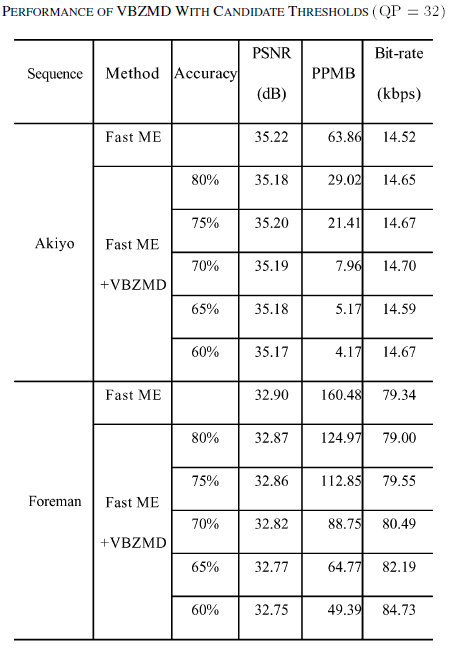
\includegraphics[width = 0.6\textwidth]{trans2-vbzmd-performance}
  \caption{参考阈值下VBZMD的表现}
  \label{fig:trans2-vbzmd-performance}
\end{figure}

直观地,高精度相对应的PSNR应该大于与低精度相对应的PSNR。然而,在这个表中可以看出,Akiyo序列中,精度为75\%对应的的PSNR值
和70\%对应的PSNR值,比精度80\%对应的PSNR高。这种情况是可能的,因为较大的阈值不仅减少了更多的计算,而且减少了编码MV所需的
比特,然后节省的比特提高了总体PSNR。

\subsubsection{可变块大小最佳运动推断}
\label{sec:vbbmd}

在减少计算量上,尽管VBZMD已经取得了相当好的表现,但我们仍可以将其改进以得到更好的表现。在H.264的中,当前块的左、上和右上
(或上左)相邻块的MV将用作预测的当前块的MV等,如 \ref{fig:trans2-neighboring-block} 所说明。由于相邻块的MV通常是相关的,
预测向量很可能正是在ME之后最好的MV。为方便描述,我们定义最佳MV为预测向量的块为预测向量块(PVB)。正如 \ref{fig:trans2-predict-vec-block} 所示,不同序列的PVB率序列是大于相应的、如 \ref{fig:trans2-zmb} 所示的 ZMB率得。特别是,对于运动较为激烈的场景,
如Coastguard和Foreman序列,PVB率较ZMB率高23\%到122\%。另一方面,另一个实验显示,对大多数序列来说,PVB率较ZMB率
高97\%。我们所观察到的现象启示我们,应当使用预测向量来预测最佳MV,而不是零MV。此外,在H.264中,进行编码和传输是
当前MV和预测矢量之间的差异,而不是当前的MV本身。因此,使用预测向量来预测最佳MV可以节省用于编码MV的比特。

\begin{figure}[H] % use float package if you want it here
  \centering
  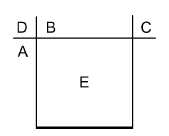
\includegraphics[width = 0.3\textwidth]{trans2-neighboring-block}
  \caption{当前块与其相邻块}
  \label{fig:trans2-neighboring-block}
\end{figure}

\begin{figure}[H] % use float package if you want it here
  \centering
  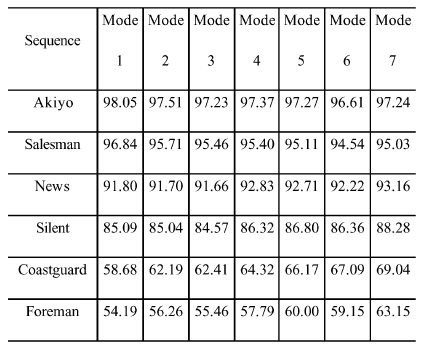
\includegraphics[width = 0.6\textwidth]{trans2-predict-vec-block}
  \caption{预测向量块比例}
  \label{fig:trans2-predict-vec-block}
\end{figure}

基于前面的VBZMD,我们提出了一种VBBMD算法。关键思想是将预测向量的成本与给定阈值进行比较。如果成本小于阈值,则将
预测向量视为最佳MV,然后可以跳过剩余的搜索点。

同样,如何选择不同块大小情况下的阈值仍然是问题的关键。使用与VBZMD中相同的方法,我们可以在不同的准确率下获得多个
候选阈值集。VBBMD的步骤与VBZMD几乎相同,唯一的区别在于,我们检查预测矢量而不是零MV。我们用候选阈值集编码不同的
视频序列,并选择最佳集合。结果表明,阈值的集合(2500, 1500, 1400,920, 625, 570,500)在准确度为66\%时提供了
一个很好的折衷。此外,模式1的低阈值THS也是800,因为它工作得很好。 \ref{fig:trans2-vbbmd} 展示出了具有最佳阈值集的VBBMD结果。
与VBZMD在同一表中的结果相比,我们可以看到,更多的搜索点被进一步减少,而PSNR和比特率几乎一样。这验证了VBBMD比VBZMD更有效。

\begin{figure}[H] % use float package if you want it here
  \centering
  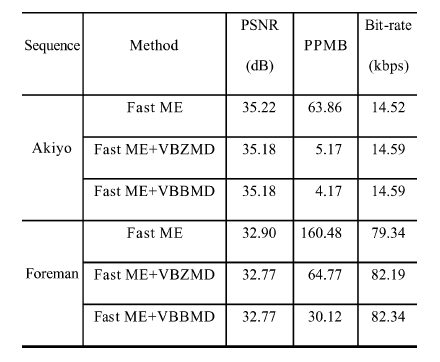
\includegraphics[width = 0.6\textwidth]{trans2-vbbmd}
  \caption{最优阈值下,VBBMD的表现(QP=32)}
  \label{fig:trans2-vbbmd}
\end{figure}

如前所述,阈值是在 $QP=32$ 的条件下确定的。然而实验表明,不同的$QP$值将得到不同的阈值。这是因为代价值$J$与$QP$
有关。在 \ref{eq2-cost} 中,$J$的值与 $\lambda$直接相关,而 $\lambda$ 的值是从一个以 $QP$ 为索引的表中查询
得到的。当一个块被视为PVB时,当前MV $\;m$ 与预测MV $\;p$ 相差最多为 $3/4$像素,这可以用10比特来编码。因此,我们
近似地设置 $R(m-p)$ 为10。我们定义 $QP=32$ 条件下的阈值为标准阈值,对于其他的 $QP$ 取值,相应的阈值应设置为
标准阈值加上 $ (\lambda_{QP} - \lambda_{32}) x 10$。

\subsection{模拟结果}
\label{sec:app2-sim-result}

我们将VBBMD实现在了H.264参考编码器上,并使用UMHexagonS快速ME算法。我们设置运动搜多范围为32,并设置
参考帧数为1。率失真优化被禁止并且CAVLC熵编码开启。

为了验证所提出的方法在不同实验条件下的有效性,我们选择了六个序列,其运动活动从小到大变化。他们是Akiyo, 
Salesman, News, Silent, Coastguard和Foreman序列。所有序列均为QCIF格式,并以30帧每秒编码。除第一帧
以外的所有帧都被编码为P帧。此外,为了检查在不同比特率下的性能,在我们的实验中使用了三个QP值:28, 32, 36。
如 \ref{sec:vbbmd} 所述,在VBBMD中使用的阈值根据QP进行调整。

为便于比较,我们在 \ref{fig:trans2-result} 中显示了平均PSNR增益($\Delta PSNR$)、PPMB平均降低率($\Delta PPMB$)
和比特率的增长率($\Delta Bit-rate$)。从结果可以看出,所提出的方法是稳定的,并且在不同的条件下工作得很好。
与仅使用快速ME算法相比,我们的方法进一步减少了76.10\%到94.12\%的整数像素搜索点,而PSNR衰减平均仅为0.06分贝,
并且比特率只是略微增加。

\begin{figure}[H] % use float package if you want it here
  \centering
  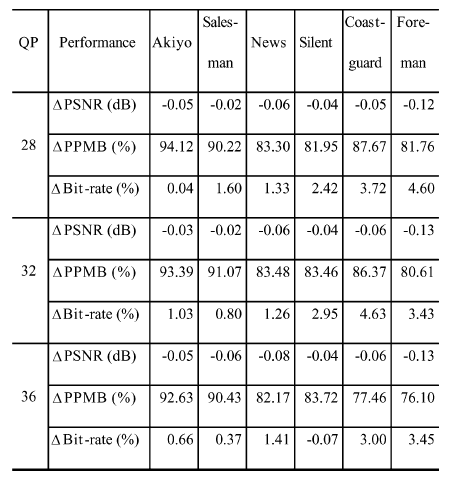
\includegraphics[width = 0.6\textwidth]{trans2-result}
  \caption{在不同条件下VBBMD的表现}
  \label{fig:trans2-result}
\end{figure}

\subsection{结论}
\label{sec:app2-conclusion}

本文提出了一种H.264视频编码的早终止方法VBBMD,该方法通过进一步减少计算总量来帮助现有的快速运动搜索
算法。该方法通过检查一个搜索点来预测最佳的MV。通过这种方法,一些运动搜索可以被提前停止,因此与这些
搜索相关联的计算可以被减少。在该方法中,考虑了复杂度的降低的同时,阈值通过基于不同块大小的检测精度来确定,
这使得阈值决策更加合理。实验结果表明,我们提出的方法实现了显著的复杂度降低,而视频质量的退化是可以忽略不计的。
未来的方向可能包括使阈值根据量化级别和运动级别自适应调整,并将早终止方法应用于子像素的运动估计。

\subsection*{References}

\begin{translationbib}
  \item Yang, Libo, et al. "An effective variable block-size early termination algorithm for H. 264 video coding." 
  IEEE Transactions on Circuits and Systems for Video Technology 15.6 (2005): 784-788.
\end{translationbib}
